\section{The Unit-Scaled Maximal Update Parametrization} \label{sec:umup}

In this section we show how \mup\ can be adapted to satisfy Unit Scaling, and provide a new set of HPs which---thanks to Unit Scaling---are more interpretable and separable than those commonly used for \mup, unlocking several practical benefits. For those wishing to apply \umup\ to their own models, we provide a user-guide in \Cref{app:using_umup_guide} and an overview of our library implementing \umup\ in \Cref{app:us_lib_guide}.

% The various challenges identified with \mup\ share a common cause: the fact that \mup\ is a parametrization (concerning \textit{relative} changes in width), not a set of \textit{absolute} rules. In this section we demonstrate that providing \mup\ with absolute scaling rules can create a foundation for addressing the problems outlined. The principle we use to do this is that of Unit Scaling, i.e. the unit variance of all activations, weights and gradients at initialization.

\subsection{Combining \mup\ with Unit Scaling} \label{sec:umup:combining_mup_with_us}

Whereas Unit Scaling provides rules for scaling all operations, \mup\ only does so for parametrized ones. It's these operations we need to address to arrive at a unified scheme, resolving differences in the scaling rules each recommends. We begin with the expressions for the $A_W,B_W,C_W$ scaling factors in \Cref{eq:abc_mup_absolute}, and substitute in the \mup\ scaling rules defined in \Cref{table:mup}. This results in a complete implementation of \mup, which is shown in the top half of \Cref{table:mup_umup_schemes} (using the \textit{extended} set of \mup\ HPs given in \Cref{table:hp_sets}). We set out to turn this into a valid Unit Scaling scheme, which requires unit initializations ($B_W \leftarrow 1$) and matmuls with the Unit Scaling factor we identified in \Cref{sec:background:unit_scaling} ($A_W \leftarrow 1/\sqrt{\fanin}$).

Our first step is to drop the $\sigma_W$ and $\basefanin$ HPs entirely, and associate the $\alpha_W$ HPs with certain functions instead of weights---decisions we justify in the rest of this section (this results in the simplified intermediate implementation in \Cref{table:mup_to_umup_1}). Our input weights now have unit initializations as desired, and a unit parameter multiplier, which is also the appropriate scaling factor (as input layers here are embedding lookups, not matmuls).

Hidden weights now have the implementation:
\begin{align} \label{eq:mup_comparison}
    A_W \leftarrow 1,
    \quad
    B_W \leftarrow \frac{1}{\sqrt{\fanin}},
    \quad
    C_W \leftarrow \eta \, \frac{1}{\fanin},
\end{align}
which differs from our Unit Scaling criteria. However, using the abc-symmetry outlined in \Cref{eq:abc_symmetry} we can shift scales by a factor of $\sqrt{\fanin}$, arriving at a unit-scaled scheme:
\begin{align} \label{eq:mup_comparison_2}
    A_W \leftarrow \frac{1}{\sqrt{\fanin}},
    \quad
    B_W \leftarrow 1,
    \quad
    C_W \leftarrow \eta \, \frac{1}{\sqrt{\fanin}}.
\end{align}
Finally, our output layers also have unit initialization, but a parameter multiplier of $A_W \leftarrow 1/\fanin$. This differs from the Unit Scaling rule, but in the forward pass this is permissible as there are no subsequent matmuls of a transformer. In the backward pass this mis-scaling would propagate, so we apply the desired $\leftarrow 1/\sqrt{\fanin}$ factor. Using different forward and backward scales in this way is usually not allowed, but is valid for output layers due to the cut-edge rule (\Cref{app:cut_edge_rule}).

The final change we make is to the input LR scaling rule, which we show in \Cref{sec:umup:emb_lr_rule} is more effective if $c_W \leftarrow 1$ is replaced with $c_W \leftarrow 1 / \sqrt{\fanout}$~\footnote{This represents a slight deviation from the Maximal Update Parametrization, though we still refer to our scheme as a form of \mup\ as it conforms in all other aspects.}. With these changes made, we arrive at our final \umup\ scheme, given in \Cref{table:mup_umup_schemes}. It's important to note that the scaling rules in this table must be combined with the standard Unit Scaling rules for other non-matmul operations. These are covered in \Cref{app:additional_unit_scaled_ops}, and implemented in our library (see \Cref{app:us_lib_guide}).

\begin{table}[t]
  \centering
  \caption{The definition of \umup\, along with an implementation of \mup\ (assuming the \textit{extended} HP set in \Cref{table:hp_sets}). \umup\ aims to simplify \mup\ and provide the benefits of Unit Scaling.}
  \vspace{0.2em}
  \label{table:mup_umup_schemes}
  \begin{tabular}{rl @{\hspace{0.8\tabcolsep}} lcccc}
      \toprule
      & \multicolumn{2}{c}{\multirow{2}{*}[-0.2em]{ABC-multiplier}} & & Weight Type \vspace{0.2em} & & \multirow{2}{*}[-0.2em]{Residual}
      \\\cline{4-6}
      \rule{0pt}{1em} & & & Input & Hidden & Output &
      \\
      \midrule
      & parameter & ($A_W$) & $\alpha_{\mathrm{emb}}$ & \hspace{1em} $1$ (or $\alpha_\mathrm{attn}$) & $\alpha_{\mathrm{out}} \frac \basefanin {\fanin}$ & $\sqrt{\frac \basedepth {\depth}}$\textsuperscript{*}
      \\
      \textbf{\mup} & initialization & ($B_W$) & $\sigma_{\mathrm{init}}$ & $\sigma_{\mathrm{init}} \sqrt{\frac \basefanin {\fanin}}$ & $\sigma_{\mathrm{init}} $ & ---
      \\
      & Adam LR & ($C_W$) & $\eta \, \hat \eta_\mathrm{emb}$ & $\eta \, \frac \basefanin {\fanin}$ & $\eta$ & $\sqrt{\frac \basedepth {\depth}}$\phantom{\textsuperscript{*}}
      \\
      \midrule
      & parameter\textsuperscript{†} & ($A_W$) & $1$ & $\frac 1 {\sqrt{\fanin}}$ & $\frac 1 {\fanin}$\textsuperscript{‡} & $\frac 1 {\sqrt{\depth}}$\textsuperscript{*}
      \rule{0pt}{1.2em}\\[0.75em]
      \textbf{\umup} & initialization & ($B_W$) & $1$ & $1$ & $1$ & ---
      \\[0.65em]
      & Adam LR & ($C_W$) & $\eta \, \frac 1 {\sqrt{\fanout}}$ & $\eta \, \frac 1 {\sqrt{\fanin}}$ & $\eta$ & $\frac 1 {\sqrt{\depth}}$\phantom{\textsuperscript{*}}
      \\[0.25em]
      \bottomrule
      \vspace{-0.4cm}
      \\
      \multicolumn{7}{l}{\small{\textsuperscript{*}Residual multipliers are applied to the end of each branch, rather than the output of linear layers.}}
      \rule{0pt}{1.2em}\\
      \multicolumn{7}{l}{\small{\textsuperscript{†}\umup's $\alpha$ HPs are associated with operations, not weights, so are not included here (see \Cref{sec:umup:principled_hps}).}}
      \\
      \multicolumn{7}{l}{\small{\textsuperscript{‡}To maintain unit scale we apply $ 1 / \sqrt{\fanin}$ scaling in the backward pass (see \Cref{app:cut_edge_rule}).}}
      \\
  \end{tabular}
  \vspace{-0.4em}
\end{table}

% Despite being a parametrization, the practical implementation of \mup\ outlined in Tensor Programs V implies a set of absolute scaling equations (table \todocite in appdx \todocite). We arrive at these by combining the basic scaling rules in \Cref{table:mup} and the final $A_W,B_W,C_W$ formulae in \Cref{eq:abc_mup_absolute}. These can be compared to the Unit Scaling rules for matmuls, which we derived in \Cref{sec:background:unit_scaling} (the key operation for which \mup\ and Unit Scaling makes competing claims are matmuls, so we do not consider others here).

% The large majority of parameters in a transformer are hidden-weights, so we consider this case first. For \mup\ we have the hidden-weight ABC rules:

% \begin{align} \label{eq:mup_comparison}
%     A_W \leftarrow \alpha_W \cdot 1,
%     \quad
%     B_W \leftarrow \sigma_W \cdot \sqrt{\frac{\basefanin}{\fanin}},
%     \quad
%     C_W \leftarrow \eta_W \cdot \frac{\basefanin}{\fanin}.
% \end{align}

% whereas Unit Scaling requires:

% \begin{align} \label{eq:us_comparison}
%     A_W \leftarrow \sqrt{\frac{1}{\fanin}},
%     \quad
%     B_W \leftarrow 1.
% \end{align}

% with any scaling of $C_W$ valid. In this form the methods are incompatible.
% Using the abc-symmetry outlined in \Cref{eq:abc_symmetry}, we can shift the scales for \mup\ in \Cref{eq:mup_comparison} by a factor of $\sqrt{\frac{\basefanin}{\fanin}}$ to obtain:
% \begin{align} \label{eq:mup_comparison_2}
%     A_W \leftarrow \alpha_W \cdot \sqrt{\frac{\basefanin}{\fanin}},
%     \quad
%     B_W \leftarrow \sigma_W \cdot 1,
%     \quad
%     C_W \leftarrow \eta_W \cdot \sqrt{\frac{\basefanin}{\fanin}}.
% \end{align}
% We then arrive at our two Unit Scaling criteria by dropping the $\alpha_W$, $\sigma_W$ and $\basefanin$ HPs (a change justified in sec \todocite). Dropping these for our input and output scaling rule results in 


% We do similarly for input and output-weights, though a shift under abc-symmetry is not required as initializations are already $\Theta(1)$.
% We emphasize that this still a valid Maximal Update Parametrization, but with the added benefit of unit-scaled tensors.
% We make three additional changes in order to improve \umup\ and address some of the difficulties identified with \mup:

% \begin{enumerate}
%     \item \textbf{Input scaling rule:} under abc-symmetry our input-weight LR scaling (with Adam) should be constant, in order to align with \mup's rules. However, in sec \todocite we show that a $\nicefrac{1}{\sqrt{\fanout}}$ rule provides better \mut\ in practice, which we incorporate into \umup~\footnote{This represents a slight deviation from the Maximal Update Parametrization, though we still refer to our scheme as a form of \mup\ as it conforms in all other aspects.}.
%     \item \textbf{Output gradient scaling:} The output parameter multiplier of $\nicefrac{1}{\fanin}$ differs from the recommended Unit Scaling rule of $\nicefrac{1}{\sqrt{\fanin}}$. This isn't a problem in the forward pass, as mis-scaling from output-weights doesn't propagate through other parts of the network. However, in the backward pass the mis-scaling of gradients does propagate. For this reason, in the case of the final readout layer we use $\nicefrac{1}{\fanin}$ in the forward pass but $\nicefrac{1}{\sqrt{\fanin}}$ in the backward. Using two different scales here is valid due to the cut-edge rule (see appdx \todocite).
%     % \vspace{0.3em}
%     % The $QK^\top$ operation also functions as a kind of output matmul, for which reason \mup\ uses $\nicefrac{1}{d_\mathrm{head}}$ scaling (rather than the usual $\nicefrac{1}{\sqrt{d_\mathrm{head}}}$, also used by Unit Scaling). We adopt the \mup\ rule, but the same cut-edge trick is not valid here. Fortunately as this operation is near the base of a residual branch the overall effect of non-unit-scaled gradients is minor.
%     \item \textbf{A different set of HPs} We also recommend the use of a different set of HPs to the ones commonly swept for \mup. We now associate the $\alpha$ multipliers in our model with functions rather than weights, never consider initialization multipliers, and in practice recommend a single global LR. This is justified in section \todocite. Later in section \todocite\ we go a step further, showing that strong results can be obtained under \umup\ dropping all HPs except the global LR.
% \end{enumerate}

% Putting this all together, we derive our final set of scaling rules, shown in \Cref{table:mup_umup_schemes}. These rules define our new scheme, which we name the Unit-Scaled Maximal Update Parametrization (\umup). For clarity, we show intermediate schemes based on the above steps in appdx \todocite. Appdx \todocite also provides explicit definitions of where each $\alpha$ HP is applied in the model.

\subsection{Out-of-the-box low-precision training} \label{sec:umup:low_prec_training}

By applying the principles of Unit Scaling to \mup, \umup\ gains a key feature: the easy use of low-precision number formats during training. We can attribute the difficulties \mup\ has with low precision to the fact that it ignores constant factors (along with weight and gradient-scaling), only ensuring that activations are \textit{of order} $\Theta(1)$. The stricter condition of unit scale across all tensors at initialization provides a way of leveraging \mup's rules in order to make low-precision training work.

%Recall that each linear module in a model induces three matrix-matrix products: one during the forward pass to compute the output and two during the backward pass, computing gradients w.r.t.~the weights and the inputs, respectively. The tensors participating in these matrix-matrix products are the input activations, the weights and the gradients w.r.t.~the output activations. If these tensors are well-scaled we can simply cast them to FP8, perform the matrix multiplication and aggregate the result in higher precision if desired, e.g. when followed by a nonlinearity.

When training a transformer model with \umup\, most scales in the model stabilize while certain tensors exhibit scale growth that potentially pushes them out of FP8 range. We empirically identify these \textit{critical tensors} to be the inputs to the attention dense projection and final FFN matmul as well as the weight of the decoder head (for details see \Cref{app:fp8_training}). The latter becomes negligible in terms of model flops as width and depth of the model increase, so we generally keep this operation in higher precision. 

Following these observations, we propose the following FP8 mixed precision scheme for \umup\ transformer models:
\begin{itemize}
    \item For non-critical matmul operations, we cast the input and weight to \texttt{E4M3}, and the gradient with respect to the output to \texttt{E5M2}. This is done in the forward computation, as well as the two backward computations (for the gradient w.r.t. the weight, respectively the input). Non-critical layers are query, key, value as well as the input layer(s) to the FFN.
    %\item In the critical matmul operations, we perform the forward matmul in higher precision (usually BF16). In the backward pass, we perform the computation for the weight gradient in higher precision as well, whereas we cast the weight and output gradient to \texttt{E4M3}, respectively \texttt{E5M2} for the input gradient computation. This is possible because only the input tensor is critical and is not used for this computation.
    \item All layers involving critical tensors, as well as embedding layer, residual addition and nonlinear functions are performed in higher precision. This also means that we directly aggregate into higher precision in each FP8 matmul. We keep optimizer states in FP32, as is usually the case in mixed precision training. 
\end{itemize}
We note that in some cases one can deal with the critical tensors by casting them to \texttt{E5M2} instead of \texttt{E4M3}, however we observed some instabilities applying this in a large scale setting, possibly due to loss of precision. In small scale scenarios we also empirically find that applying the \texttt{E4M3} format instead of \texttt{E5M2} for the gradients is possible, but becomes problematic in a more realistic setting where gradients require a higher dynamic range. 

With our proposed mixed precision scheme, about $70$\% of the matmul computations in the transformer block are performed natively in FP8 (assuming a standard architecture, e.g. Llama). If desired, a dynamic per-tensor scaling could still be applied to the critical tensors.


%and require a separate treatment in order to be cast to lower precision. The two solutions we propose here are either to use the \texttt{E5M2} format to represent the larger scales or to apply a dynamic rescaling of the matmul input (\Cref{sec:experiments:fp8} and \Cref{subsec:large_scale} respectively).  

% We now turn our attention to the remaining challenges identified with \mup, showing how \umup addresses them.

\subsection{A principled approach to hyperparameters} \label{sec:umup:principled_hps}

We saw in \Cref{sec:challenges:which_hps} that approaches for selecting which HPs to sweep are poorly motivated in the literature. Our objective in \umup\ is to find a simple, well-justified and effective alternative. To this end, we propose the following ideal criteria:

\begin{enumerate}
    \item \textbf{Minimal cardinality}: the use of as few HPs as possible.
    \item \textbf{Maximal expressivity}: the ability to still express any model defined using the per-tensor $\alpha_W, \sigma_W, \eta_W$ HPs outlined in \Cref{sec:background:the_maximal_update_parameterization} (in practice, we relax this slightly).
    \item \textbf{Minimal interdependency}: the optimal value of each HP should not depend on the value of other HPs, simplifying the search space.
    \item \textbf{Interpretability}: there should be a clear explanation for what an HP's value `means' in the context of the model.
\end{enumerate}

\begin{wraptable}{r}{17.6em}
    \vspace{-0.75em}
    \caption{Typical transformer HPs used under different schemes. \textit{Basic} HPs in \textbf{bold} are considered most impactful and are commonly swept. \textit{Extended} HPs in non-bold are not always swept, often set heuristically or dropped.}
    \label{table:hp_sets}
    \vspace{-1em}
    \begin{tabular}{ccc}\\\toprule  
        SP & \mup\ & \umup\ \\\midrule
        {$\boldsymbol{\eta}$} & {$\boldsymbol{\eta}$} & {$\boldsymbol{\eta}$}
        \\ 
        $\sigma\text{-}\mathrm{scheme}$ & $\boldsymbol{\sigma_\mathrm{init}}$ &
        \\
          & $\boldsymbol{\alpha_\mathrm{emb}}|\boldsymbol{\eta_\mathrm{emb}}$ & $\alpha_\mathrm{ffn\text{-}act}$
        \\
          & $\alpha_\mathrm{attn}$ & $\alpha_\mathrm{attn\text{-}softmax}$
        \\
          & $\alpha_\mathrm{out}$ & $\alpha_\mathrm{res}$
        \\
          & $\basewidth$ & $\alpha_\mathrm{res\text{-}attn\text{-}ratio}$
        \\
          & $\basedepth$ & $\alpha_\mathrm{loss\text{-}softmax}$
        \\
        \bottomrule
    \end{tabular}
    \vspace{-2em}
\end{wraptable}

The \umup\ HPs given in \Cref{table:hp_sets} are designed to satisfy these criteria, to the fullest extent possible. The placement of these HPs in the model is given in \Cref{tab:ops_compendium}.

\paragraph{Cardinality \& expressivity} We arrive at our set of HPs in three steps, starting with the full $\alpha_W, \sigma_W, \eta_W$ for each weight tensor $W$. Firstly, we can choose to `drop' any one of these three HPs by permuting under abc-symmetry, such that one HP $=1$. As we want our weights to begin with unit scale, we choose $\sigma_W$ (i.e. $\theta = \sigma_W$ in \Cref{eq:abc_symmetry}), leaving just $\alpha_W, \eta_W$.

Secondly, we observe that several of the $\alpha_W$ HPs combine linearly with other $\alpha_W$ HPs, providing an opportunity to re-parametrize with a single HP. For instance, we noted in \Cref{sec:the_challenges_with_mup_in_practice} that the scale of self-attention softmax activations is proportional to the product of $\sigma_W$ multipliers, and the same is true for $\alpha_W$ multipliers: $\operatorname{std}(x_\mathrm{attn}) \propto \alpha_{W_\mathrm{Q}}\alpha_{W_\mathrm{K}}$. In this instance it appears more natural to use a single $\alpha$ parameter and associate it with the attention operation, rather than the weights. We term this $\alpha_\mathrm{attn\text{-}softmax}$.

We apply the same principle to the rest of the model, associating $\alpha$ HPs with operations instead of weights. This applies to all operations, unless they are unary and $k$-homogeneous for $k \ge 0$, in which case they propagate scale and don't require an HP (see \Cref{app:non-homogeneous}). This results in the set of HPs shown, with their placement in the model given in \Cref{tab:ops_compendium}.
% As desired, the scheme at this point is maximally expressive, which we prove in appdx \todocite. 

Thirdly, we use a single global $\eta$ and group $\alpha$ HPs across layers. This breaks our expressivity criterion, but we argue represents the best trade-off between expressivity and cardinality. We show in \Cref{app:umup_lr_mults} that having tuned a global $\eta$ HP and our extended $\alpha$ HPs, the further benefits of tuning per-tensor $\hat{\eta}_W$ HPs (which modify the global $\eta$) is minimal, justifying our decision to only use one global $\eta$.

\paragraph{Interdependency}

The second stage above, moving $\alpha$ HPs from weights into subsequent operations, not only reduces the number of HPs, but also minimizes the interdependence between those that remain. Interactions between HPs are complex and unlikely to be entirely separable, but we find that \umup's optimal HP values depend less on each other than under \mup\ (see \Cref{sec:experiments:hp_independence}).

\paragraph{Interpretability} 

The combination of unit scale and reduced dependencies between HPs means that each $\alpha$ can be interpreted as determining some fundamental property of the model at initialization. For example, the $\alpha_\mathrm{loss\text{-}softmax}$ HP defines the (inverse of) the softmax's \textit{temperature} for a unit-scaled input. We also introduce a new scaling scheme (defined in \Cref{subsubsec:umup_residual_in_full}) for residual connections, designed to give HPs independence and a clear interpretation: $\alpha_\mathrm{res}$ defines the contribution of the residual connections to the output scale, and $\alpha_\mathrm{res\text{-}attn\text{-}ratio}$ defines the relative contribution of attention versus FFN branches.
Finally, we choose not to include base shape HPs in \umup. They do not add to expressivity, lack a clear interpretation (besides alignment to a base model at a particular shape), break the interpretations of other HPs (as given above), and complicate implementation.

\subsection{A new embedding LR rule} \label{sec:umup:emb_lr_rule}

Although theoretical transfer properties have been proved for \mup, not all its HPs have had \mut\ shown empirically. We do so for the \textit{extended} \mup\ transformer HPs in \Cref{{fig:experiments:hp_transfer_over_width}}, where we observe poor transfer across width for the embedding LR multiplier $\hat{\eta}_\mathrm{emb}$. The associated scaling rule for the embedding LR is constant in width ($c_\mathrm{emb} = 1$), but this poor multiplier transfer suggests the rule is mis-specified. We show in \Cref{fig:umup:emb_lr_rule} (left) that a more effective rule is $c_\mathrm{emb} = 1 / \sqrt{\fanout}$. 

This keeps the optimal value of $\hat{\eta}_\mathrm{emb}$ the same regardless of width. \Cref{fig:umup:emb_lr_rule} (right) shows that a constant scaling rule leads to diminishing returns as width increases, whereas our new rule continues to work well at scale, attaining the same loss at 2048-width that constant scaling attains at 4096-width.
Our adoption of this change is a key factor in the improved performance of \umup\ over \mup\ in \Cref{fig:fig1}. 
We offer no theoretical justification for our rule, which we leave to further work.
% (possibly building on the alignment analysis of \citep{Scaling_Exponents}).

\begin{figure}[t]
    \centering
    \begin{subfigure}{\textwidth}
        \centering
        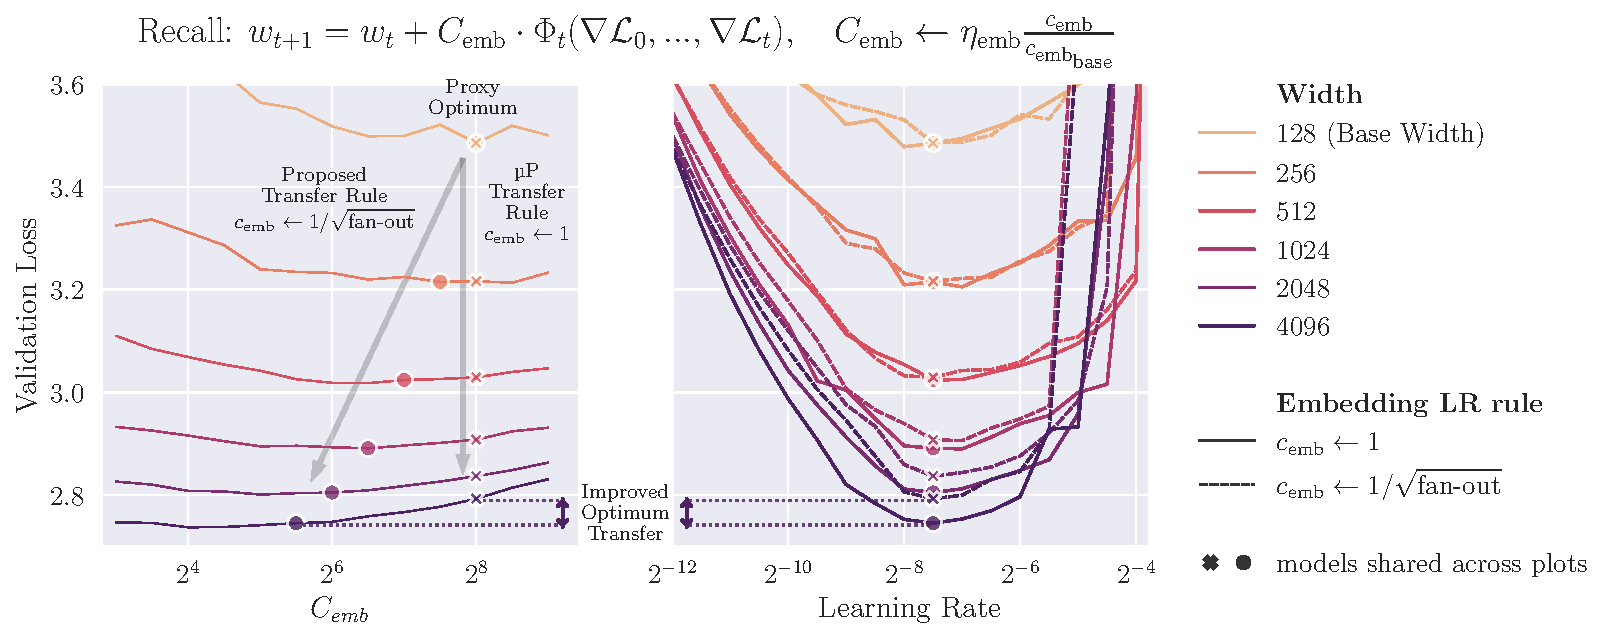
\includegraphics[width=\textwidth]{arXiv/figures/fig_embeddingLR.pdf}
    \end{subfigure}
    \caption{(Left) holding the embedding LR ($\hat{\eta}_\mathrm{emb}$) constant, vs. scaling with $\sqrt{\nicefrac{\basewidth}{\mathrm{width}}}$, both with a fixed global LR. This suggests the \mup\ embedding LR rule ($c_\mathrm{emb}$) should follow the latter scaling. (Right) we test this by sweeping the global LR under the two scaling rules. The new rule leads to lower loss on large models. (Dot/cross markers represent the same runs across both graphs).}
    \label{fig:umup:emb_lr_rule}
\end{figure}

\subsection{Hyperparameter search} \label{sec:umup_hp_search}

As shown in section \Cref{sec:background:the_maximal_update_parameterization}, the standard approach to HP search for \mut\ is via a random sweep over all HPs simultaneously. Sweeping individual HPs separately is challenging due to the dependencies between them. In contrast, \umup's HPs are designed to admit such a strategy due to our interdependence criterion. Because of this, we propose a simpler sweeping strategy for \umup\ which we term \textit{independent search} (outlined in detail in \Cref{app:umup_hp_search_algorithm}).

Independent search involves a sweep of the LR, followed by a set of one-dimensional sweeps of the other HPs (which can be run in parallel). The best results from the individual sweeps are combined to form the final set of HP values. We also consider an even simpler scheme, which only sweeps the LR, leaving other HP values at 1 (i.e. dropping them). For caution, we recommend the full approach, but in practice we find that only sweeping the LR is surprisingly effective, as shown in \Cref{fig:fig1} (a). This indicates that not only is the principle of unit scale good for numerics, but also for learning dynamics where it provides near-optimal scaling.
